% !TeX root = thesis.tex

\chapter{Proposed framework: \velocity{}}
\label{chap:velocity}

The implementation part of this thesis consists of a framework and a set of tools, tailored at optimising the test suite as well as providing accompanying metrics and insights. The framework was named \emph{\velocity{}} to reflect its purpose of enhancing the speed at which \CI{} is practised. This paper will now proceed by outlining the design goals of the framework. Afterwards, a high-level schematic overview of the implemented architecture will be provided, followed by a more in-depth explanation of every pipeline step. In the final section of this chapter, the \emph{Alpha} algorithm will be presented. This prioritisation algorithm was constructed by combining various ideas of aforementioned algorithms.

% !TeX root = ../thesis.tex

\section{Design goals}
\velocity{} has been implemented with four design goals in mind:
\begin{enumerate}
	\item \textbf{Extensibility:} It should be possible and straightforward to support additional CI systems, programming languages and test frameworks. Similarly, a clear interface must be provided to integrate new prioritisation algorithms.
	
	\item \textbf{Minimally invasive:} Integrating \velocity{} into an existing test suite should not require drastic changes to any of the test cases.
	
	\item \textbf{Language agnosticism:} This design goal is related to the extensibility of the framework. The implemented tools should not need to be aware of the programming language of the source code, nor the used test framework.
	
	\item \textbf{Self-improvement:} The prioritisation framework must support multiple algorithms. However, the performance of an algorithm might be dependent on the nature of the source code. An algorithm may offer a very high accuracy on one project but fall short on another. The framework should decide by itself which algorithm it should prefer, by measuring the performance of a prediction and subsequently infer which algorithm to use for future predictions.
\end{enumerate}
% !TeX root = ../thesis.tex

\section{Architecture}

\begin{figure}[htbp!]
	\centering
	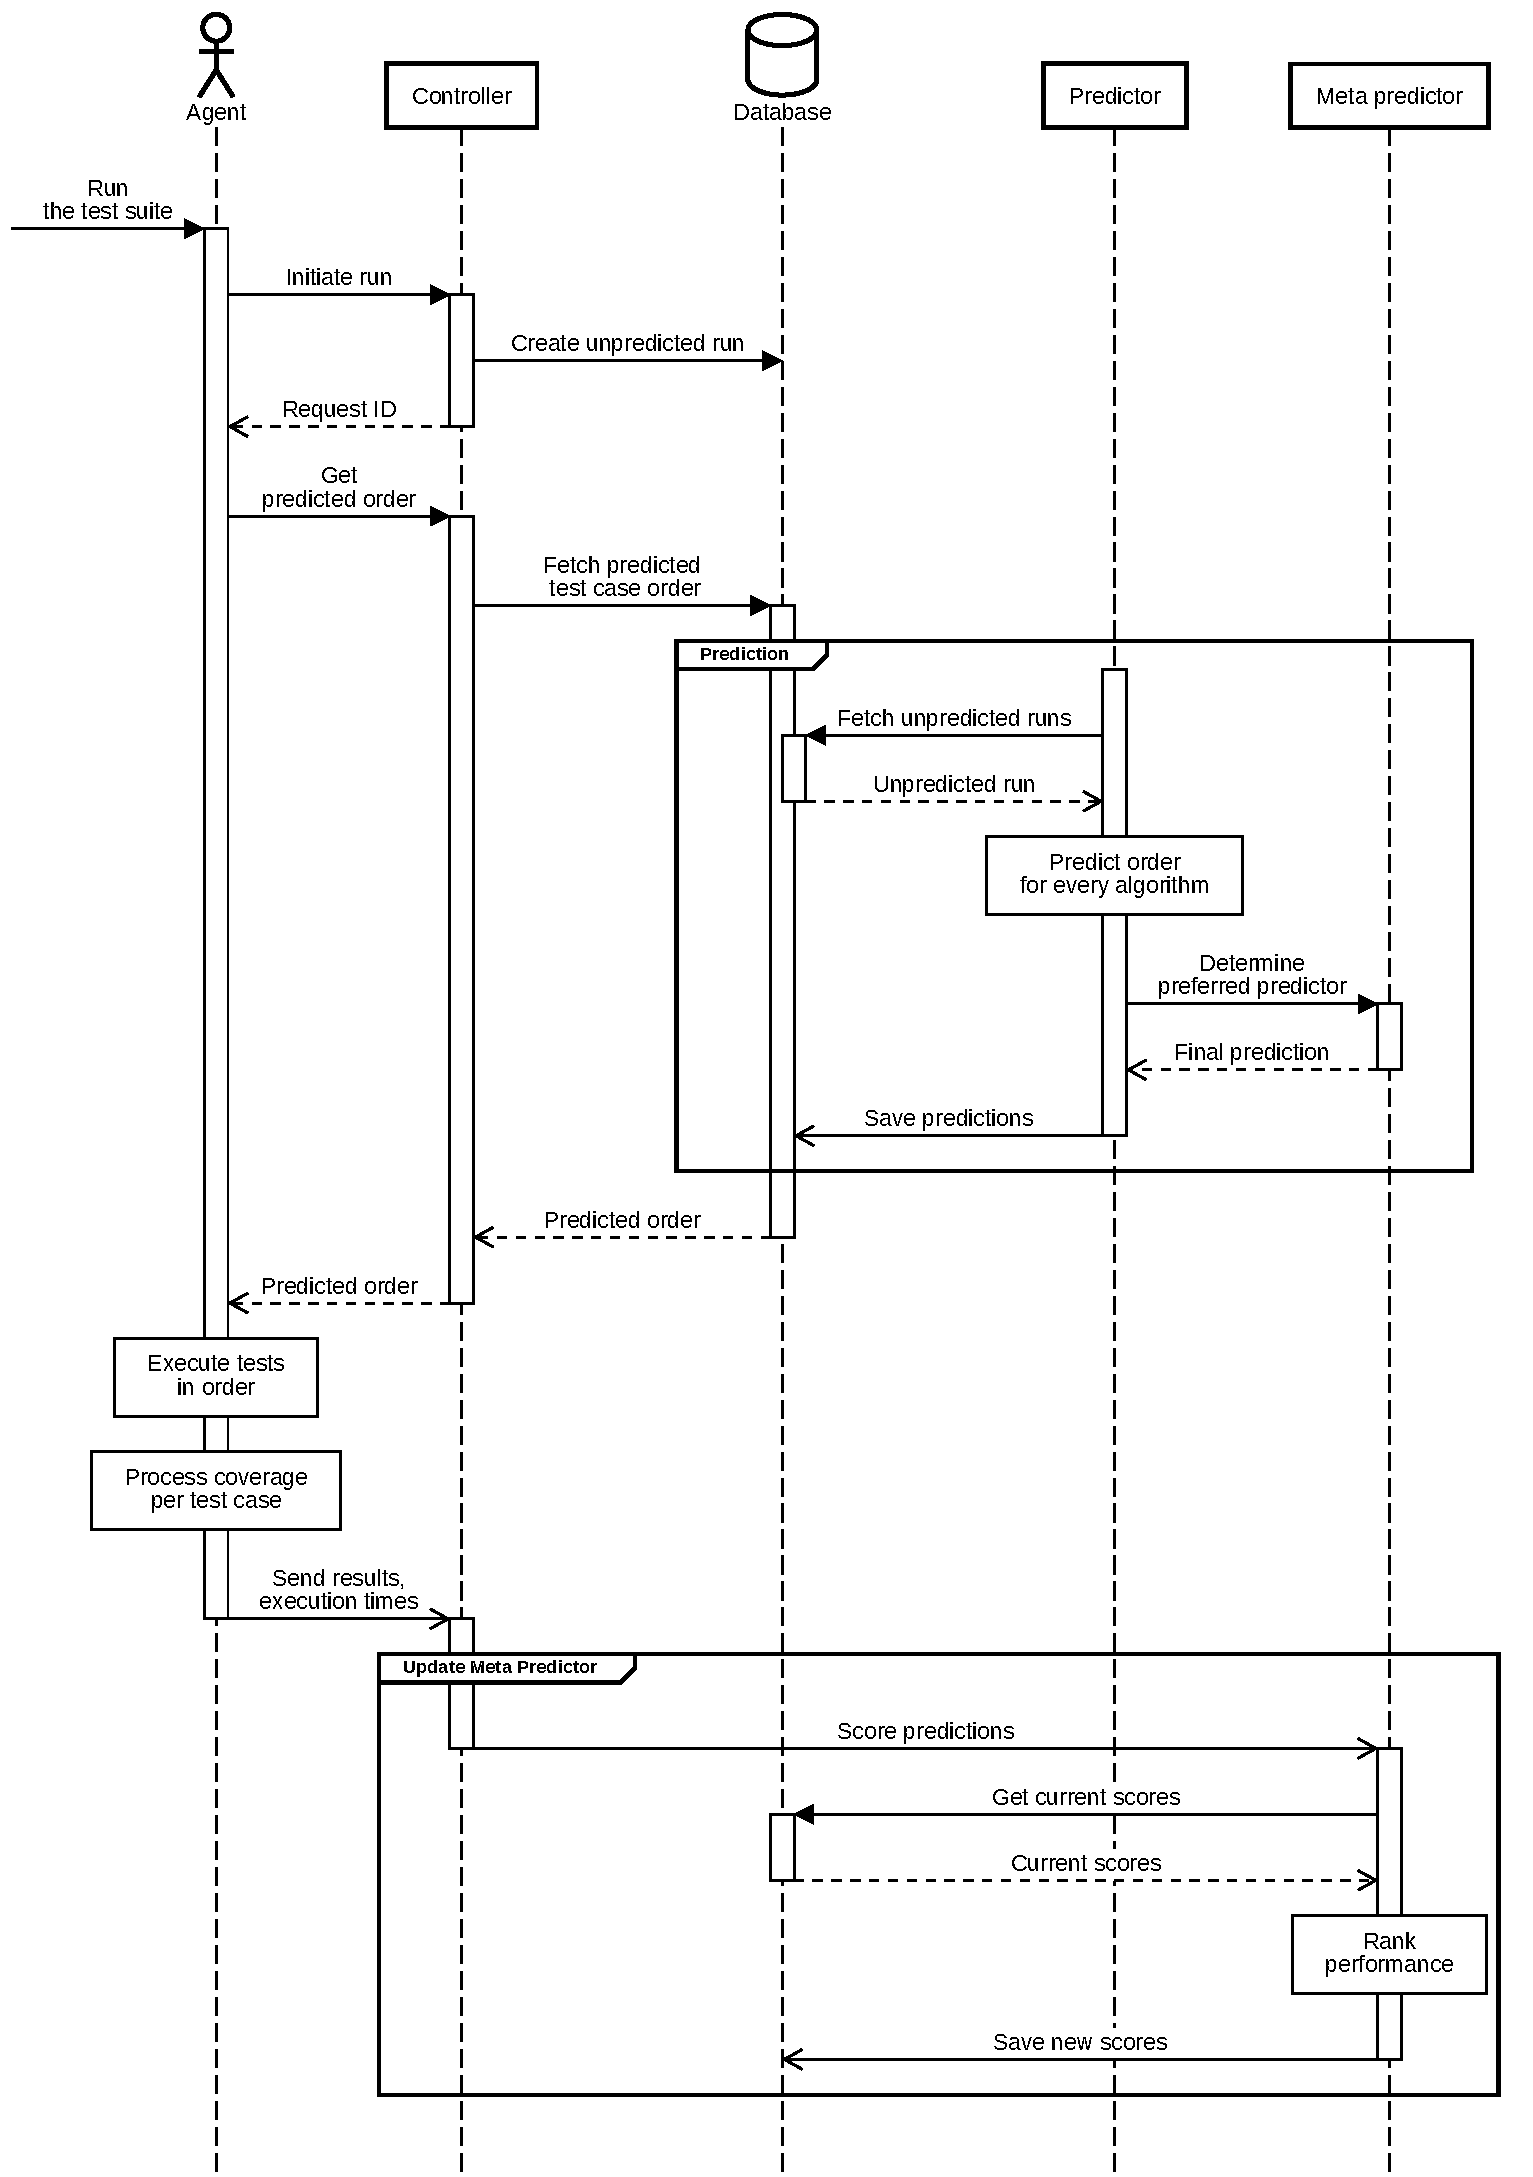
\includegraphics[height=\textheight]{assets/diagrams/sequence-diagram.pdf}
	\caption{Sequence diagram of \velocity{}}
	\label{fig:velocity-sequence-diagram}
\end{figure}

\subsection{Agent}
\label{ssec:velocity-frontend}
The first component that we will consider is the agent. The agent interacts directly with the source code and the test suite and is, therefore, the only component that is specific to the programming language and the test framework. Every programming language and test framework requires a different implementation of the agent, although these implementations are strongly related. This thesis provides a Java agent, which is available as a plugin for the Gradle and JUnit test framework, a combination which has previously been described in \cref{ssec:relatedwork-gradle-junit}. When the test suite is started, the plugin will contact the controller (\cref{ssec:velocity-controller}) to obtain the prioritised test case order and subsequently execute the test cases in that order. Afterwards, the plugin will send a feedback report to the controller, where it is analysed.

\subsection{Controller}\label{ssec:velocity-controller}
The second component is the core of the framework, acting as an intermediary between the agent on one side and the predictor (\cref{ssec:velocity-predictor}) on the other side. In order to satisfy the second design goal and as such allow language agnosticism, the controller exposes a \Gls{rest}-interface, to which the agent can communicate using the \texttt{HTTP} protocol. On the other side, the controller does not communicate directly with the predictor but stores prediction requests in a shared database instead. The predictor will periodically poll this database and update the request with the predicted order. Besides providing routing functionality between the agent and the predictor, the controller is additionally responsible for updating the meta predictor (\cref{ssec:pipeline-postanalysis}) by evaluating the accuracy of earlier predictions.

\subsection{Predictor and Metrics}\label{ssec:velocity-predictor}
The final component is the predictor. The predictor is responsible for applying the prioritisation algorithms to predict the optimal execution order of the test cases. This order is calculated by first executing ten prioritisation algorithms and subsequently consulting the meta predictor to determine the preferred sequence. The predictor has been implemented in Python, because of its accessibility and compatibility with various existing libraries such as NumPy\footnote{\url{https://numpy.org/}} and TensorFlow\footnote{\url{https://www.tensorflow.org/}}, to allow advanced prioritisation algorithms. 
% !TeX root = ../thesis.tex

\section{Pipeline}
This section will elaborate on the individual steps of the pipeline. The steps will be discussed by manually executing the pipeline that has hypothetically been implemented on a Java project. For the sake of simplicity, this explanation will assume a steady-state situation, ensuring the existence of at least one completed run of this project in the database at the controller side.

\subsection{Initialisation}\label{ssec:pipeline-initialisation}
As was explained before, the provided Java implementation of the agent was designed to be used in conjunction with Gradle. In order to integrate \velocity{} into a Gradle project, the build script (\texttt{build.gradle}) should be modified in two places. The first change is to include and apply the plugin in the header of the file. Afterwards, the plugin requires three properties to be configured:
\begin{itemize}
	\item \texttt{base} the path to the Java source files, relative to the location of the build script. This will typically resemble \texttt{src/main/java}.
	
	\item \texttt{repository} the url to the git repository at which the project is hosted. This is required in subsequent steps of the pipeline, to detect which code lines have been changed in the commit currently being analysed.
	
	\item \texttt{server} the url at which the controller can be reached.
\end{itemize}

\noindent \autoref{lst:pipeline-buildgradle} contains a minimal integration of the agent in a Gradle build script, applied to a library for generating random numbers\footnote{\url{https://github.com/thepieterdc/random-java}}. The controller is hosted at the same host as the agent and is accessible at port \texttt{8080}.

\lstinputlisting[caption=Minimal Gradle buildscript, label=lst:pipeline-buildgradle, language=Groovy]{assets/listings/build.gradle}

\noindent After the project has been configured, the test suite must be executed. For the Gradle agent, this involves executing the built-in \texttt{test} task. This task requires an additional argument to be passed, which is the commit hash of the changeset to prioritise. In every discussed \CI{} system, this commit hash is available as an environment variable.\\

\noindent The first step is for the agent to initiate a new test run in the controller. This is accomplished by sending a \texttt{POST}-request to the \texttt{/runs} endpoint of the controller, which will reply with an identifier. On the controller side, this request will result in a new prioritisation request being enqueued in the database that will asynchronously be processed by the predictor daemon in the next step.

\subsection{Prediction}
The prediction of the test execution order is performed by the predictor daemon. This daemon continuously polls the database to fetch new test runs that need to be predicted. When a new test run is detected, the predictor executes every available prediction algorithm in order to obtain multiple prioritised test sequences. The following algorithms are available:

\paragraph*{AllInOrder} The first algorithm will simply prioritise every test case alphabetically and will be used for for benchmarking purposes in \autoref{chap:evaluation}.

\paragraph*{AllRandom} The second algorithm has also been implemented for benchmarking purposes. This algorithm will ``prioritise'' every test case arbitrarily.

\paragraph*{AffectedRandom} This algorithm will only consider the test cases that cover source code lines which have been modified in the current commit. These test cases will be ordered randomly, followed by the other test cases in the test suite in no particular order.

\paragraph*{GreedyCoverAll} The first of three implementations of the Greedy algorithm (\autoref{ssec:alg-greedy}) will execute the algorithm to prioritise the entire test suite.

\paragraph*{GreedyCoverAffected} As opposed to the previous greedy algorithm, the second Greedy algorithm will only consider test cases covering changed source code lines to be prioritised. After these test cases, the remaining test cases in the test suite will be ordered randomly.

\paragraph*{GreedyTimeAll} Instead of greedily attempting to cover as many lines of the source code using as few tests as possible, this implementation will attempt to execute as many tests as possible, as soon as possible. In other words, this algorithm will prioritise test cases based on their average execution time.

\paragraph*{HGSAll} This algorithm is an implementation of the algorithm presented by Harrold, Gupta and Soffa (\autoref{ssec:alg-hgs}). It is executed for every test case in the test suite.

\paragraph*{HGSAffected} Similar to the \emph{GreedyAffected} algorithm, this algorithm is identical to the previous \emph{HGSAll} algorithm besides that it will only prioritise test cases covering changed source code lines.

\paragraph*{ROCKET} The penultimate algorithm is a straightforward implementation of the pseudocode provided in \autoref{ssec:alg-rocket}.

\paragraph*{Alpha} The final algorithm has been inspired by the other implemented algorithms. \autoref{sec:velocity-alpha} will further elaborate on the details.\\

\noindent Subsequently, the final prioritisation order is determined by applying the meta predictor. Essentially, the meta predictor can be seen as a table which assigns a score to every algorithm, indicating its performance on this codebase. \autoref{ssec:pipeline-postanalysis} will explain later how this score is updated. The predicted order by the algorithm with the highest score is eventually elected by the meta predictor as the final prioritisation order, and saved to the database.

\subsection{Test case execution}
Regarding the agent, the identifier obtained in \autoref{ssec:pipeline-initialisation} is used to poll the controller by sending a \texttt{GET} request to \texttt{/runs/id}, which will reply with the test execution order if this has already been determined. One of the discussed features of Gradle in \autoref{ssec:relatedwork-gradle-junit} was the possibility to execute test cases in a chosen order by adding annotations. However, this feature cannot be used to implement the Java agent, since it only supports ordering test cases within the same test class. In order to facilitate complete control over the order of execution, a custom \texttt{TestProcessor} and \texttt{TestListener} have been implemented.\\

\noindent The \texttt{TestProcessor} is responsible for processing every test class in the classpath and forward it along with configurable options to a delegate processor. The final processor in this chain will eventually perform the actual execution of the test class. Since the delegate processors that are built into Gradle will by default execute every method in the test class, the custom processor needs to work differently. The implemented agent will first store every received test class into a list and load the class to obtain all test cases in the class using reflection. After all classes have been processed, the processor will iterate over the prioritised order. For every test case $t$ in the order, the delegate processor is called with a tuple of the corresponding test class and an options array which excludes every test case except $t$. This will effectively forward the same test class multiple times to the delegate processor, but each time with an option that restricts test execution to the prioritised test case, resulting in the desired behaviour.\\

\noindent Subsequently, the \texttt{TestListener} is a method that is called before and after every invocation of a test case. This listener allows the agent to calculate the duration of every test case, as well as collect the intermediary coverage and save this on a per-test case basis.

\subsection{Post-processing and analysis}\label{ssec:pipeline-postanalysis}
The final step of the pipeline is to provide feedback to the controller, to evaluate the accuracy of the predictions and thereby implementing the fourth design goal of self-improvement. After executing all test cases, the agent sends the test case results, the execution time and the coverage per test case to the controller by issuing a \texttt{POST} request to \texttt{/runs/id/test-results} and \texttt{/runs/id/coverage}.\\

\noindent Upon receiving this data, the controller will update the meta predictor using the following procedure. The meta predictor is only updated if at least one of the test cases has failed, since the objective of \tcp{} is to detect failures as fast as possible, thus every prioritised order is equally good if there are no failures at all. If however a test case did fail, the predicted orders are inspected to calculate the duration until the first failed test case for every order. Subsequently, the average of all these durations is calculated. Finally, the score of every algorithm that predicted a below average duration until the first failure is increased, otherwise it is decreased. This will eventually lead to the most accurate algorithms being preferred in subsequent test runs.
% !TeX root = ../thesis.tex

\section{Alpha algorithm}
Besides the algorithms which have been presented in \autoref{sec:relatedwork-algorithms}, an additional algorithm has been implemented: the \emph{Alpha} algorithm. This was constructed by examining the philosophy behind every discussed algorithm and subsequently combining the best ideas into a novel prioritisation algorithm. The specification below will assume the same naming convention as described in \autoref{def:alg-naming}. The pseudocode is provided in Algorithm \ref{alg:alpha}\\

\noindent The algorithm consumes the following inputs:
\begin{itemize}
	\item the set of all $n$ test cases: $TS = \{T_1, \dots, T_n\}$
	
	\item the set of $m$ \emph{affected} test cases: $AS = \{T_1, \dots, T_m\} \subseteq TS$. A test case $t$ is considered ``affected'' if any source code line which is covered by $t$ has been modified or removed in the commit that is being predicted.
	
	\item $C$: the set of all lines in the application source code, for which a test case $t \in TS$ exists that covers this line and that has not yet been prioritised. Initially, this set contains every covered source code line.
	
	\item the failure status of every test case, for every past execution out of $k$ executions of that test case: $F = \{F_1, \dots, F_n\}$, where $F_i = \{f_1, \dots, f_k\}$. $F_{tj} = 1$ implies that test case $t$ has failed in execution $current - j$.
	
	\item the execution time of test case $t \in TS$ for run $r \in [1 \dots k]$, in milliseconds: $D_{tr}$.
	
	\item for every test case $t \in TS$, the set $TL_t$ is composed of all source code lines that are covered by test case $t$.
\end{itemize}

\noindent The first step of the algorithm is to determine the execution time $E_t$ of every test case $t$. This execution time is calculated as the average of the durations of every successful (i.e.) execution of $t$, since a test case will be prematurely aborted upon the first failed assertion, which introduces bias in the duration timings. In case $t$ has never been executed successfully, the average is computed over every execution of $t$.

\[
	E_t = \left.
	\begin{cases}
		\overline{\{D_{ti} \vert i \in [1 \dots k], F_{ti} = 0\}} & \exists j \in [1 \dots k], F_{tj} = 0 \\
		\overline{\{D_{ti} \vert i \in [1 \dots k]\}} & \text{otherwise} \\
	\end{cases}
	\right.
\]

\noindent Next, the algorithm executes every affected test case that has also failed at least once in its three previous executions. This reflects the behaviour of a developer attempting to resolve the bug that caused the test case to fail. Specifically executing \emph{affected} failing test cases first is required in case multiple test cases are failing and the developer is resolving these one by one, an idea which was extracted from the ROCKET algorithm (\autoref{ssec:alg-rocket}). In case there are multiple affected failing test cases, the test cases are prioritised by increasing execution time. After every selected test case, $C$ is updated by subtracting the code lines that have been covered by at least one of these test cases.\\

\noindent Afterwards, the same operation is repeated for every failed but unaffected test case, likewise ordered by increasing execution time. Where the previous step helps developers to get fast feedback about whether or not the specific failing test case they were working on has been resolved, this step ensures that other failing test cases are not forgotten and are executed early in the run as well. Similar to the previous step, $C$ is again updated after every prioritised test case.\\

\noindent Research (TODO reference) has indicated that on average, only a small fraction (TODO PERCENTAGE \%) of all test runs will contain failed tests, resulting in the previous two steps not being executed at all. Therefore, the most time should be dedicated to executing test cases that cover affected code lines. More specifically, the next step of the algorithm executes every affected test case, sorted by decreasing cardinality of the intersection between $C$ and the lines which are covered by the test case. Conforming to the prior two steps, $C$ is also updated to reflect the selected test case. As a consequence of these updates, the cardinalities of these intersections change after every update, which will ultimately lead to affected tests not strictly requiring to be executed. This idea has been adopted from the Greedy algorithm \autoref{ssec:alg-greedy}.\\

\noindent In the penultimate step, the previous operation is repeated in an identical fashion for the remaining test cases, similarly ordered by the cardinality of the intersection with the remaining uncovered lines in $C$.\\

\noindent Finally, the algorithm selects every test case which had not yet been prioritised. Notice that these test cases do not contribute to the test coverage, as every test case that would incur additional coverage would have been prioritised already in the previous step. Subsequently, these test cases are actually redundant and are therefore candidates for removal by \tsm{}. However, since this is a prioritisation algorithm, these tests will still be executed and prioritised by increasing execution time.

\begin{algorithm}[h!]
\caption{Alpha algorithm for \tcp{}}
\label{alg:alpha}
\begin{algorithmic}[1]
	\State {\bfseries Input:} Set $TS = \{T_1, \dots, T_n\}$ of all test cases,
	
	Set $AS = \{T_1, \dots T_m\} \subseteq TS$ of affected test cases,
	
	Set $C$ of all source code lines that are covered by any $t \in TS$,
	
	Execution times $D_{tr}$ of every test case $t$, over all $k$ runs $r$ of that test case,
	
	Failure status $FS$ for each test case over the previous $m$ successive iterations,
	
	Sets $TL = \{TL_1, \dots, TL_n\}$ of all source code lines that are covered by test case $t \in TS$.
	
	\State {\bfseries Output:} Ordered list $P$ of $n$ test cases and their priorities.
	\State $P \gets array[1 \dots n]$ \Comment{initially $0$}
	\State $i \gets n$
	\State $FTS \gets \{t \vert t \in TS \wedge (F[t][1] = 1 \vee F[t][2] = 1 \vee F[t][3] = 1)\}$
	\State $AFTS \gets AS \cap FTS$
	
	\ForAll{$t \in AFTS$} \Comment{sorted by execution time in $E$ (ascending)}
		\State $C \gets C \setminus TL[t]$
		\State $P[t] \gets i$
		\State $i \gets i - 1$
	\EndFor
	
	\State $FTS \gets FTS \setminus AFTS$
	\ForAll{$t \in FTS$} \Comment{sorted by execution time in $E$ (ascending)}
		\State $C \gets C \setminus TL[t]$
		\State $P[t] \gets i$
		\State $i \gets i - 1$
	\EndFor
	
	\State $AS \gets AS \setminus FTS$
	\While{$AS \neq \emptyset$}
		\State $t\_max \gets AS[1]$ \Comment{any element from $AS$}
		\State $tl\_max \gets \emptyset$
		
		\ForAll{$t \in AS$}
			\State $tl\_current \gets C \cap TL_{t}$
			\If{$|tl\_current| > |tl\_max|$}
				\State $t\_max \gets t$
				\State $tl\_max \gets tl\_current$
			\EndIf
		\EndFor
		
		\State $C \gets C \setminus tl\_max$
		\State $P[t] \gets i$
		\State $i \gets i - 1$
	\EndWhile
	
	\State $TS \gets TS \setminus (AS \cup FTS)$
	\While{$TS \neq \emptyset$}
		\State $t\_max \gets TS[1]$ \Comment{any element from $TS$}
		\State $tl\_max \gets \emptyset$
		
		\ForAll{$t \in TS$}
			\State $tl\_current \gets C \cap TL_{t}$
			\If{$|tl\_current| > |tl\_max|$}
				\State $t\_max \gets t$
				\State $tl\_max \gets tl\_current$
			\EndIf
		\EndFor
		
		\State $C \gets C \setminus tl\_max$
		\State $P[t] \gets i$
		\State $i \gets i - 1$
	\EndWhile
	\Return $P$
	
\end{algorithmic}
\end{algorithm}